% ~ 6 pages
\chapter{The ATLAS Experiment at the Large Hadron Collider}
\label{chap:atlas}

The LHC at CERN is a symmetric proton--proton and heavy ion collider, supplying
collision events to four major experiments: ATLAS, CMS, ALICE and LHCb. In
proton--proton operation, bunches of protons are crossed at the interaction
points located inside of the experiments with a peak bunch crossing rate
of~\SI{40}{\mega\hertz}~\cite{lhc}. With a proton beam energy of \SI{6.5}{\TeV}
during Run~2 of the LHC, the proton--collisions take place at a center-of-mass
energy of \SI{13}{\TeV}. During the 2016 data taking period, a peak
instantaneous luminosity of~\SI{1.4e34}{\per\square\centi\metre\per\second} was
reached~\cite{lhc_2016_report}, which was further increased for the 2017 period.

\section{The ATLAS Detector}
\label{sec:atlas}

The ATLAS detector~\cite{atlas_detector} is a multipurpose particle detector
experiment at the LHC. An overview of the detector is given in
Figure~\ref{fig:atlas_detector}. Its cylindrical geometry provides almost
$4\pi$~coverage of the nominal interaction point with a forward-backward
symmetry. Specialised detector subsystems are arranged in concentric layers
around the beam axis, enabling the reconstruction of photons, electrons, muons,
taus and jets. Moreover, the detector coverage allows to reconstruct missing
transverse energy from weakly and non-interacting particles.

\begin{figure}[htb]
  \centering
  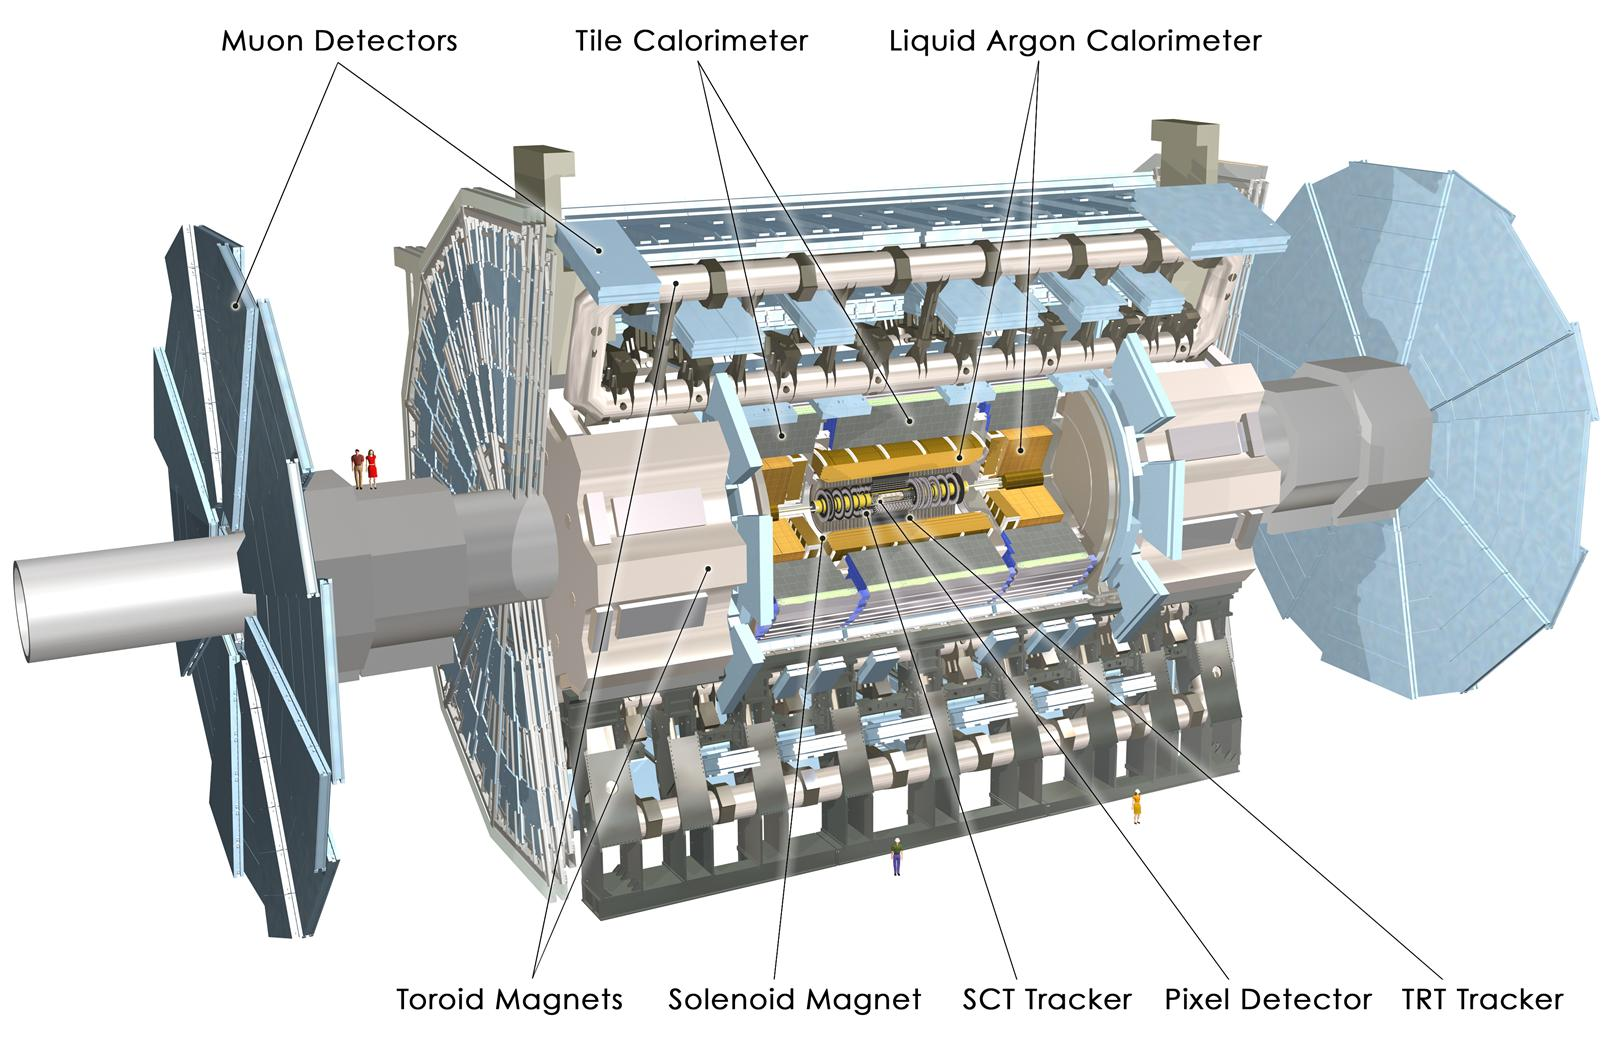
\includegraphics[width=0.8\textwidth]{./figures/atlas/overview.jpg}
  \caption{Overview of the ATLAS detector~\cite{atlas_detector}. Shown is the
    inner detector consisting of pixel, microstrip (SCT), transition radiation
    tracker (TRT) and solenoid; the calorimeter system consisting of LAr and
    Tile sampling calorimeters and the muon spectrometer consisting of tracking
    chambers and air-core toroids.}
  \label{fig:atlas_detector}
\end{figure}

In the ATLAS experiment a right-handed coordinate system is used to describe
positions in the detector. The origin of the coordinate system is located at the
nominal interaction point, with the $z$-axis pointing along the beam axis, the
$x$-axis towards the centre of the LHC ring and the $y$-axis upwards. The $x$-
and $y$-axes span the transverse plane. Spherical
coordinates~$(\rho, \varphi, \theta)$ are commonly used, with the azimuthal
angle~$\varphi$ being measured in the transverse plane and the polar
angle~$\theta$ with respect to the beam axis.

Due to the unknown longitudinal momentum of colliding partons in the
proton--proton collisions, the momentum of final state particles only balances
in the transverse plane. Therefore, transverse quantities for momentum and
energy are defined as
\begin{align*}
  p_\text{T} &= |\mathbf{p}| \sin\theta & E_\text{T} &= E \sin\theta \eqdot
\end{align*}
In addition, the unknown boost along the $z$-axis motivates the definition of
the pseudorapidity
\begin{align*}
  \eta &= -\ln\left[ \tan\left( \frac{\theta}{2} \right) \right] \eqcomma
\end{align*}
such that differences in~$\eta$ are Lorentz-invariant in the massless limit, and
the angular distance
\begin{align*}
  \Delta R &= \sqrt{\left(\Delta\eta\right)^2 + \left(\Delta\varphi\right)^2} \eqcomma
\end{align*}
where $\Delta \eta$ and $\Delta \varphi$ are the differences in pseudorapidity
and azimuthal angle, respectively.

In the following a brief description of the detector subsystems is given. In
increasing radial distance, the systems are:
\begin{description}
\item[Inner Detector] The inner detector (ID) consists of several layers of
  pixel detectors, silicon microstrip detectors and straw chambers. The ID is
  embedded in a \SI{2}{\tesla} axial magnetic field, bending the trajectories of
  charged particles in the transverse plane and allowing transverse momentum
  measurements. Hits of charged tracks in the active layers of the ID are
  reconstructed as space points, which are used to perform tracking and
  vertexing. The straw tubes of the Transition Radiation Tracker (TRT) offer
  large radius tracking as well as electron identification via high-threshold
  hits originating from transition radiation of electrons crossing the tube
  material.

\item[Calorimeter] The sampling calorimeters used in the ATLAS detector allow to
  measure the energies of photons, electrons and hadrons. The calorimeter system
  consists of an electromagnetic calorimeter with high granularity, designed to
  reconstruct energy depositions of photons and electrons, and the coarser
  hadronic calorimeter to reconstruct jets of hadrons.

\item[Muon Spectrometer] Muons passing the calorimeter are measured in
  high-precision tracking chambers in the magnetic field of an air-core toroid.
  The spectrometer allows to identify muons and measure their momentum from the
  curvature of reconstructed tracks in the muon system.

\item[Trigger System] The peak event rate of \SI{40}{\mega\hertz}, mostly
  consisting of events not of immediate interest for physics research, needs to
  be reduced in the trigger system to match the limited throughput of the data
  acquisition systems. The trigger system is divided into three levels: L1, L2
  and the event filter, which successively reduce the rate while having access
  to detector information of increasing granularity. The rate after the event
  filter allows moving the events to permanent storage for later analysis.
\end{description}
For the reconstruction of hadronic tau decays, the tracking and calorimeter
systems are of large importance. They are described in more detail in the
following.

\subsection{Inner Detector}
\label{sec:atlas_tracking}

\begin{figure}[ht]
  \centering
  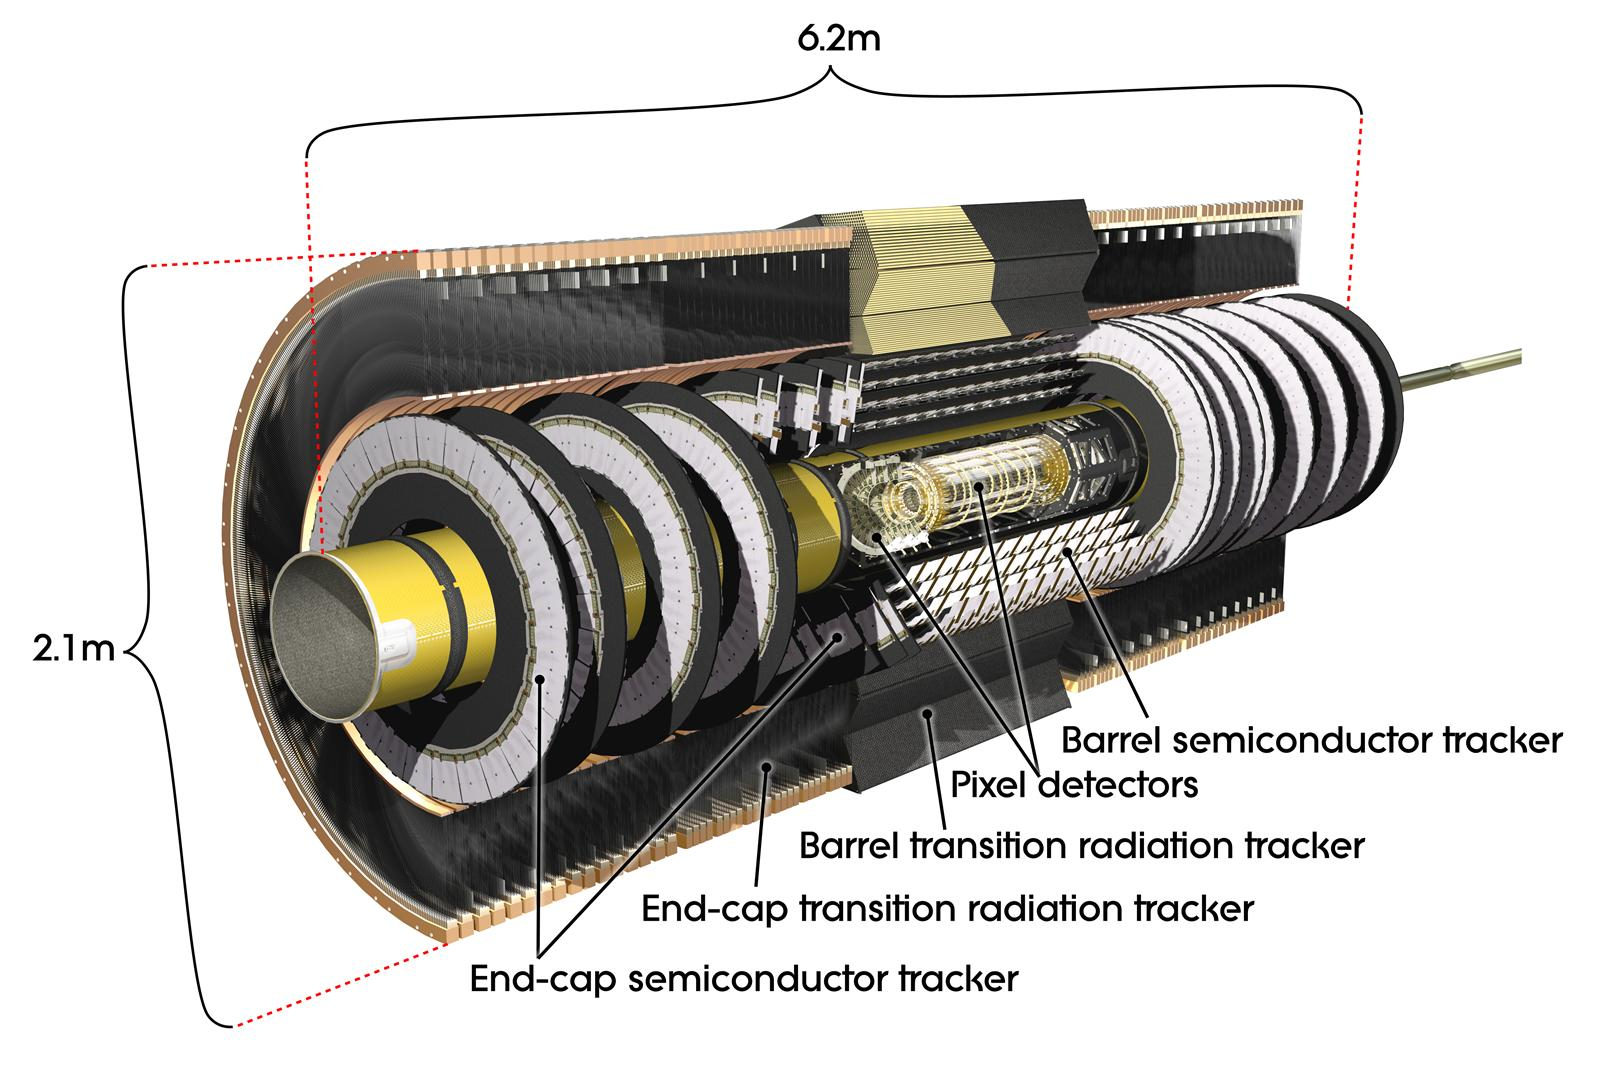
\includegraphics[width=0.75\textwidth]{./figures/atlas/inner_detector.jpg}
  \caption{ATLAS inner detector\cite{indet_fig} also in \cite{atlas_detector}.
    Not shown IBL!}
  \label{fig:atlas_indet}
\end{figure}

Accurate track reconstruction: tracking in high particle densities, meet
momentum and vertex resolution requirements

Three subparts: pixel, sct, trt

IBL: installed during LS1, reduce distance to the IP (33mm), whats that good
for? r= 33.25 mm

Pixel includes IBL

Pixel: Three layers in barrel and endcap, intrinsic resolution 10mu in rphi,
115mu in z, r=50.5mm to 122.5mm

SCT: silicon strip modules, four barrel layers and two endcaps with 9 layers
each, r=299mm to 514mm

TRT: gas-filled straw tubes, barrel and two endcaps, 130mu intrinsic resolution in rphi,
r=554mm to 1082mm


\todo[inline]{Introduce abbrev.\ IBL}
\todo[inline]{Define impact parameter: $d_0$ and $z_0$.}
\todo[inline]{Define perigee}
% See \url{https://twiki.cern.ch/twiki/bin/view/AtlasProtected/InDetTrackingDC14#Impact_parameters_z0_d0_definiti}

Coverage to $|\eta| < 2.5$

\todo[inline]{Find primary sources on this stuff!}
\begin{itemize}
\item Track \& vertex reconstruction
\item Charged particles provide hits in ID
\item High spacial resolution to reconstruct tracks in dense environments
  (number of tracks per event -- 200? -- check this)
\item Solenoid field with \SI{2}{\tesla}
\item Secondary vertex reconstruction (B-layer -- this is important, Pixel, SCT)
\item TRT -- 'continuous' tracking (what is this?) and distinction between
  electrons and hadrons using transition-radiation
\item ID acceptance $|\eta| < \num{2.5}$
\item Split into barrel and two endcap regions
\item Pixel: Three barrel layers, three endcap layers each (and 1 layer IBL).
  Pixel detector in 'Pixel Support Tube' to allow exchange of elements in case
  of radiation damage. Inner Radius \SI{4.2}{\centi\metre} and outer radius
  \SI{25}{\centi\metre}.
\item The layer after the IBL is called B-layer!
\item IBL \cite{ibl_tdr}: Improve B-tagging when modules in the remaining pixel layers fail;
  Tracking inefficiencies at high pileup affects B-layer needs redundancy;
  Better impact parameter reconstruction improves vertexing and b-tagging
\item Pixel layers segmented in $r\varphi$ and $z$. Single pixel
  \SI{50}{\micro\metre} in $r\varphi$ and \SI{400}{\micro\metre} in $z$
\item Silicon strip detectors (four layers) in support structure with radius of
  about \SI{55}{\centi\metre}
\item SCT strip detectors \SI{15}{\micro\metre} $r\varphi$ and
  \SI{70}{\micro\metre} $z$ resolution
\item TRT: Barrel region $|\eta| < \num{0.5}$, on average a track causes 36
  hits; Resolution decreases with pile-up
\end{itemize}

\subsection{Calorimeter System}
\label{sec:atlas_calo}

\todo[inline]{Topoclustering}
\todo[inline]{Define what a moment is}
\todo[inline]{EM and LC scale}
\todo[inline]{Introduce nomenclature: strip layer, EM1, EM2, EM3, HAD}

Coverage:

EM LAr covers $|\eta|< 3.2$

Scintillator-tile in~$|\eta| < 1.7$

End-caps hadronic $|\eta| > 1.5$ also LAr coverage to $|\eta| = 4.9$

\begin{figure}[ht]
  \centering
  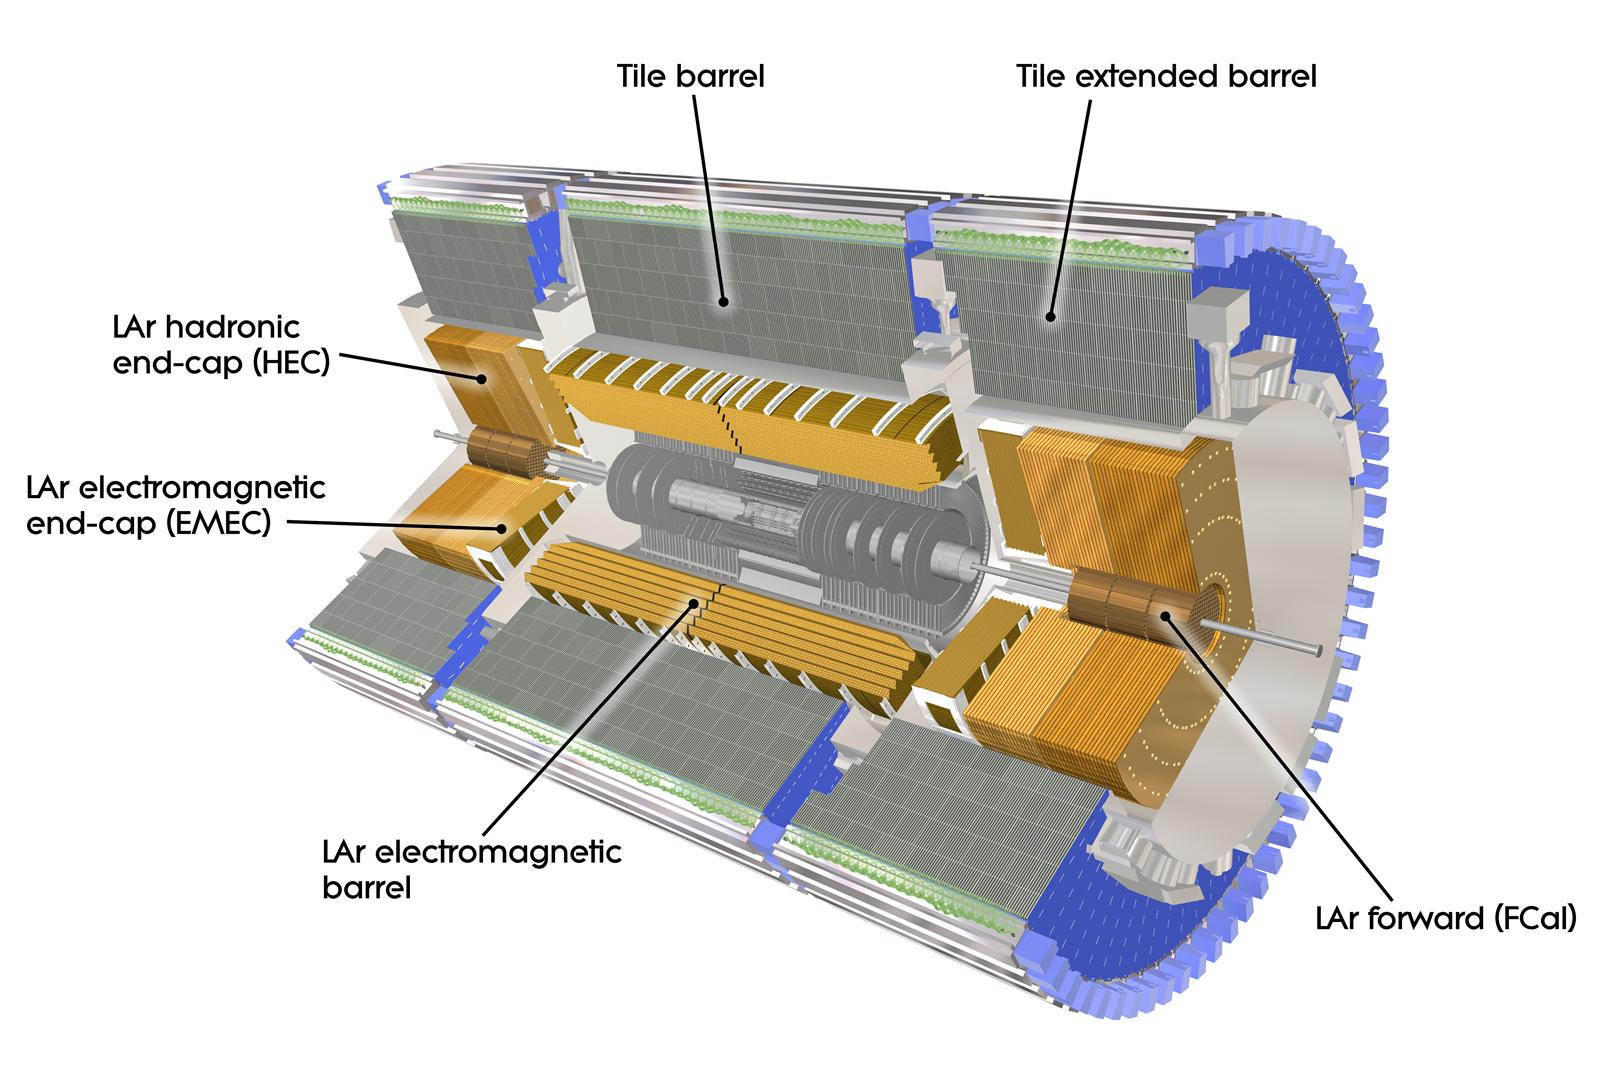
\includegraphics[width=0.8\textwidth]{./figures/atlas/calorimeter.jpg}
  \caption{ATLAS calorimeter\cite{calo_fig} also in \cite{atlas_detector}}
  \label{fig:atlas_indet}
\end{figure}



\begin{itemize}
\item LHC (brief)

\item ATLAS
  \begin{itemize}
  \item Overview (Design goals) \\
    brief: Beam Line, Inner Detector \& Solenoid, Calorimeter, Muon System \&
    Toroid, Trigger

  \item Nomenclature (Coordinate system, Pseudorapidity, $\Delta R$,
    $p_\mathrm{T}$)

  \item Inner detector / Tracker (and why they are important for taus)
    \begin{itemize}
    \item Pixel, IBL
    \item SCT
    \item TRT
    \item  Transverse Momentum Resolution, Vertex \& Secondary Vertex
      reconstruction, Impact Parameter Resolution, $\eta$-Coverage
    \end{itemize}

  \item Calorimeter (and why they are important for taus)
    \begin{itemize}
    \item Presampler, LAr (EM1 - EM3), Had (Tile, LAr)
    \item Cell sizes, $\eta$-Coverage, Thickness $X_0$ / $\lambda$,
      Energy Resolution vs. $E$
    \item Topoclusters \& Cluster moments
    \end{itemize}

  \end{itemize}
\end{itemize}

%%% Local Variables:
%%% mode: latex
%%% TeX-master: "mythesis"
%%% End:
